\documentclass[final,hyperref={pdfpagelabels=false}]{beamer}

\mode<presentation>{\usetheme{I6pd2_hugo}}
\usepackage[english]{babel}
\usepackage[utf8]{inputenc}
\usepackage{amsmath,amsthm, amssymb, latexsym, subfigure}
%\usepackage{times}\usefonttheme{professionalfonts}  % obsolete
%\usefonttheme[onlymath]{serif}
\boldmath
\usepackage[orientation=portrait,size=a0,scale=1.4,debug]{beamerposter}
% change list indention level
% \setdefaultleftmargin{3em}{}{}{}{}{}
\usecaptiontemplate{
\small
\structure{\insertcaptionname~\insertcaptionnumber:}
\insertcaption
}


%\usepackage{snapshot} % will write a .dep file with all dependencies, allows for easy bundling

\usepackage{array,booktabs,tabularx,subfigure,graphicx}
\newcolumntype{Z}{>{\centering\arraybackslash}X} % centered tabularx columns
\newcommand{\pphantom}{\textcolor{ta3aluminium}} % phantom introduces a vertical space in p formatted table columns??!!

\listfiles

%%%%%%%%%%%%%%%%%%%%%%%%%%%%%%%%%%%%%%%%%%%%%%%%%%%%%%%%%%%%%%%%%%%%%%%%%%%%%%%%%%%%%%
 
\title{	Evaluation of the Beam Coupling Impedance of New Beam Screen Designs for the LHC Injection Kicker Magnets}
\author{H. Day\thanks{hugo.day@hep.manchester.ac.uk}$^{\dagger\ddagger\star}$, M.J. Barnes$^{\dagger}$, F. Caspers$^{\dagger}$, R.M. Jones$^{\ddagger \star}$, E. Metral$^{\dagger}$, B. Salvant$^{\dagger}$ \\
$\dagger$ CERN, Switzerland \\
$\ddagger$ School of Physics and Astronomy, The Univeristy of Manchester, Manchester, UK \\
$\star$ Cockcroft Institute, Daresbury, UK \\}
\date[May 14th 2013]{May 14th 2013}

%%%%%%%%%%%%%%%%%%%%%%%%%%%%%%%%%%%%%%%%%%%%%%%%%%%%%%%%%%%%%%%%%%%%%%%%%%%%%%%%%%%%%%
\newlength{\columnheight}
\setlength{\columnheight}{105cm}


%%%%%%%%%%%%%%%%%%%%%%%%%%%%%%%%%%%%%%%%%%%%%%%%%%%%%%%%%%%%%%%%%%%%%%%%%%%%%%%%%%%%%%
\begin{document}
\begin{frame}
  \begin{columns}
    % ---------------------------------------------------------%
    % Set up a column 
    \begin{column}{.49\textwidth}
      \begin{beamercolorbox}[center,wd=\textwidth]{postercolumn}
        \begin{minipage}[T]{.95\textwidth}  % tweaks the width, makes a new \textwidth
          \parbox[t][\columnheight]{\textwidth}{ % must be some better way to set the the height, width and textwidth simultaneously
            % Since all columns are the same length, it is all nice and tidy.  You have to get the height empirically
            % ---------------------------------------------------------%
            % fill each column with content            
            \begin{block}{Abstract}
\small{
The LHC injection kicker magnets (MKIs) have experienced a significant degree of beam induced heating since the beginning of 2011 due to the increasing intensity stored in the LHC, for long periods of time, and the relatively large broadband beam coupling impedance of the installed kicker magnets. In this paper we show the sources of impedance in the MKIs, and the effect that the beam screen dimensions have on the impedance. We show how these alter the power loss, and present an improved beam screen design that improves shielding of the magnet, whilst further improving the electrical breakdown situation.
}
\end{block}
            \vfill

	\begin{block}{Introduction}
\small{
\begin{figure}
\subfigure[]{
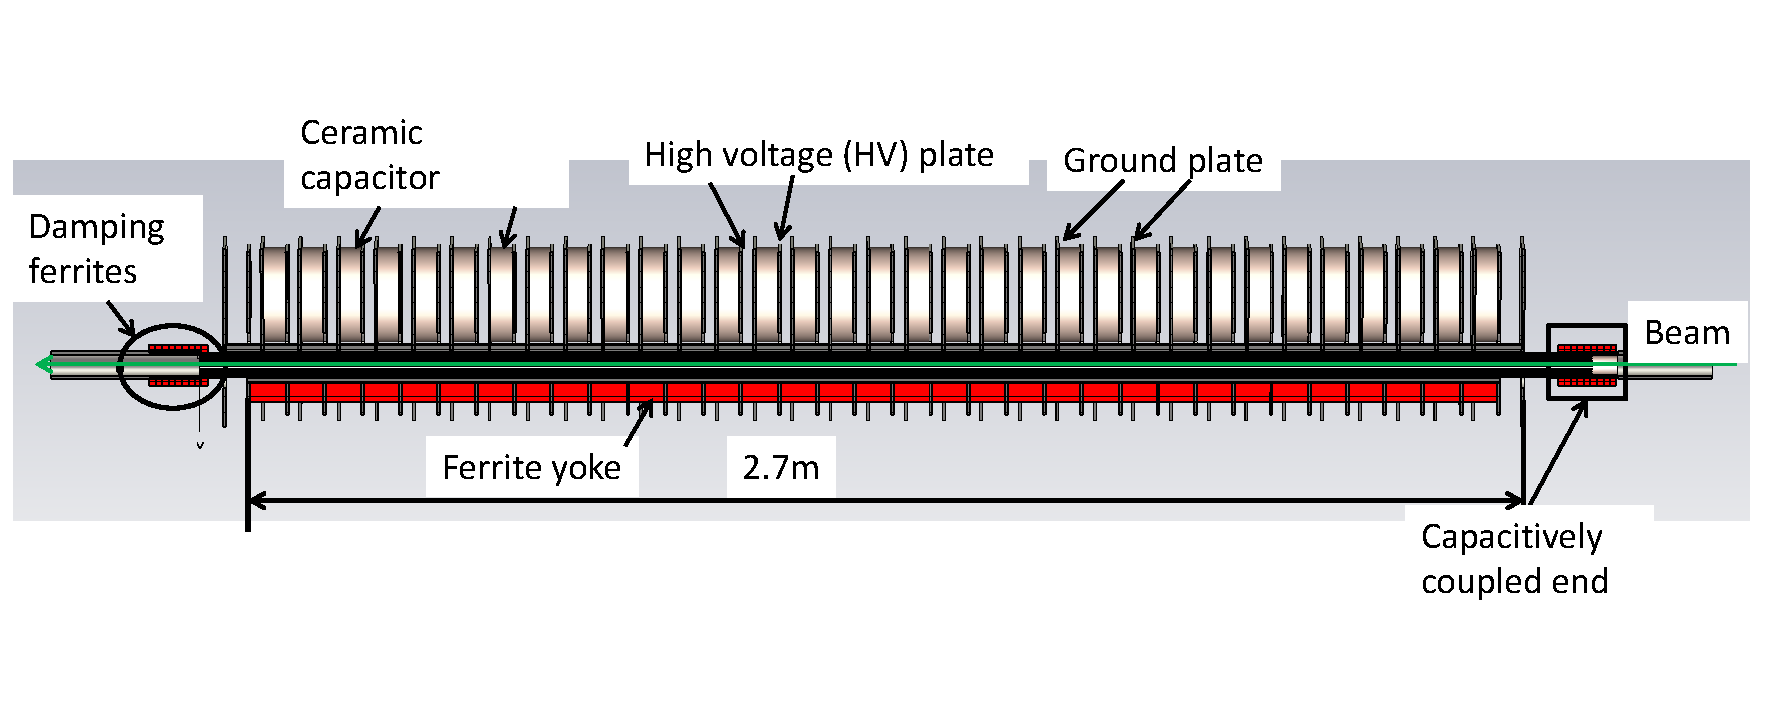
\includegraphics[width=0.5\textwidth]{MKICrossSectionYZ.pdf}
\label{fig:mkiStruct}
}
\subfigure[]{
\includegraphics[width=0.45\textwidth]{internalStruct.jpg}
\label{fig:SideView}
}
\caption{\subref{fig:mkiStruct} The structure of the MKI and \subref{fig:SideView} the internal structure of the beam screen.}

\end{figure}

	\begin{itemize}
	\item{During operation of the LHC in 2011 and 2012, high temperatures were observed in the LHC injection kicker magnets (MKIs), becoming higher as the bunch intensity was increased to reach higher luminosities [1].}
	\item{The heating was determined to be caused by beam-induced heating due to the circulating beam interacting with the real component of the longitudinal beam coupling impedance in the magnet. The hottest magnet before technical stop 3 (TS3), MKI8D, was replaced with a new beam screen in TS3 to improve the screening of the ferrite yoke (structure shown in Fig.~\ref{fig:mkiStruct}).}
	\item{The improved screening was shown to be highly effective, strongly reducing the temperature of MKI8D, seen in Fig.~\ref{fig:HeatingPt8}, where it can be seen MKI8D changes from being the hottest magnet at IP8 to the coldest after TS3 [2].}

	\end{itemize}
\begin{figure}
\subfigure[]{
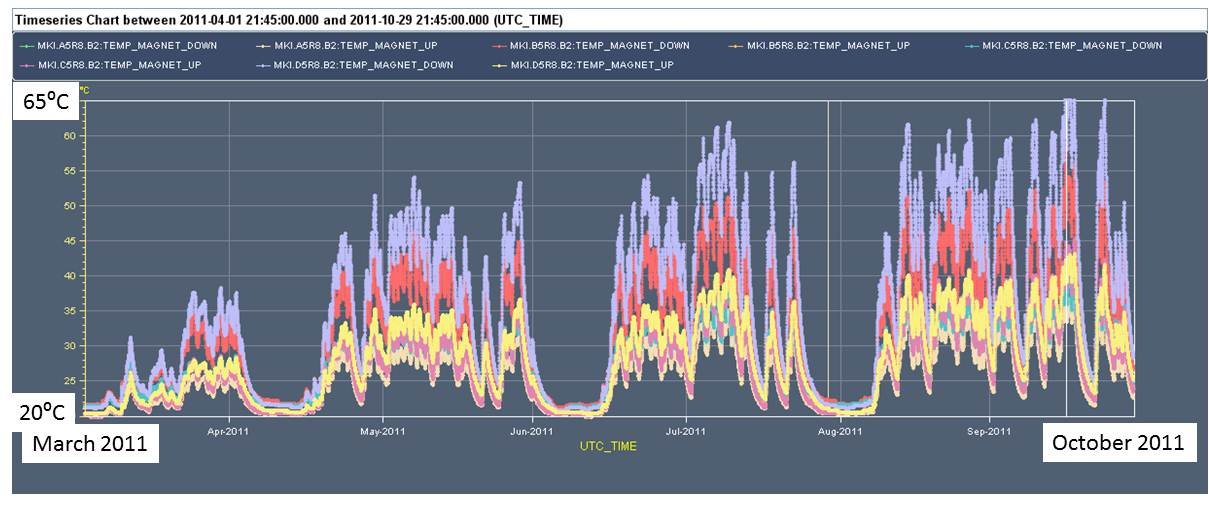
\includegraphics[width=0.5\textwidth]{mkipt8HeatingBefore.jpg}
\label{fig:point8Before}
}\\
\subfigure[]{
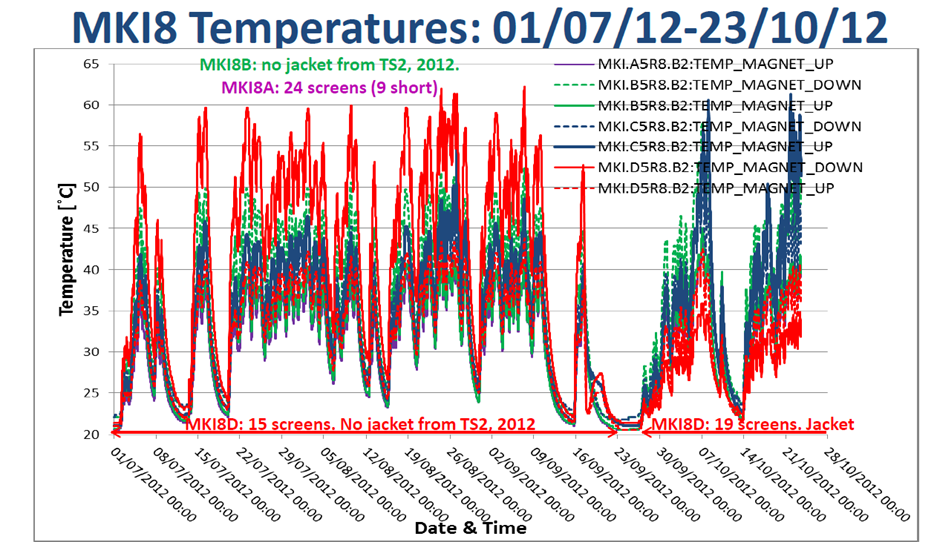
\includegraphics[width=0.5\textwidth]{mki8-temps-post-ts3.png}
\label{fig:point8After}
}
\caption{Heating of the MKIs at IP8 before \subref{fig:point8Before} and after \subref{fig:point8After} TS3.}
\label{fig:HeatingPt8}
\end{figure}
}
	\end{block}
 \vfill
\begin{block}{New Beam Screen Design}
\small{
\begin{itemize}
\item{A new screen design has been proposed [3] for installation in the MKIs during long shutdown 1 (LS1) which aims to include 24 screen conductors in the design, whilst lowering the surface electric field on the ceramic tube during kicker pulsing, shown in Fig.~\ref{fig:newScreenDesign}.}


\begin{figure}
\includegraphics[width=0.45\textwidth]{mki-final-design.pdf}
\caption{The proposed beam screen design for the MKI post-LS1.}
\label{fig:newScreenDesign}
\end{figure}

\item{The capacitively coupled end is significantly changed:}
\begin{itemize}
\item{The external metallization is replaced by an external metal tube which steps away from the ceramic tube near the ends of the screen conductors. This reduces the surface electric field on the ceramic tube significantly. Tapering the length of the conductors also helps this reduction.}
\item{This reduction allows 24 screen conductors to be placed back in the beam screen, greatly improving the screening of the ferrite yoke from the beam.}
\end{itemize}
\item{In addition the thermal emissivity of the inside of the vacuum tank is planned to be increased to help improve heat evacuation from the tank.}
\end{itemize}
}
\end{block}
            \vfill


           \vfill
         \vfill
          }
        \end{minipage}
      \end{beamercolorbox}
    \end{column}
    % ---------------------------------------------------------%
    % end the column

    % ---------------------------------------------------------%
    % Set up a column 
    \begin{column}{.49\textwidth}
      \begin{beamercolorbox}[center,wd=\textwidth]{postercolumn}
        \begin{minipage}[T]{.95\textwidth} % tweaks the width, makes a new \textwidth
          \parbox[t][\columnheight]{\textwidth}{ % must be some better way to set the the height, width and textwidth simultaneously
            % Since all columns are the same length, it is all nice and tidy.  You have to get the height empirically
            % ---------------------------------------------------------%
            % fill each column with content

\vfill

\begin{block}{Beam Coupling Impedance of the New Screen Design}
\small{
\begin{itemize}
\item{To acquire the beam coupling impedance of the proposed design the structure was simulated using CST Particle Studio [4].}
\item{The longitudinal impedance is simulated for 3 cases; the beam screen before TS3 for all MKIs, the screen for the revised MKI8D installed during TS3, and the proposed screen design for post LS1. The real components of all are shown in Fig.~\ref{fig:MKIScreenImp}}

\end{itemize}

\begin{figure}
\subfigure[]{
\includegraphics[width=0.4\textwidth]{realImp.pdf}
\label{fig:MKIScreenImp}
}
\subfigure[]{
\includegraphics[width=0.4\textwidth]{mki-overlap-len-real-imp-zoom.pdf}
\label{fig:mkiOverlapRes}
}
\caption{\subref{fig:MKIScreenImp} The real component of the longitudinal beam coupling impedance of the existing MKIs, the replacement MKI8D and the proposed beam screen design for after LS1. \subref{fig:mkiOverlapRes} The resonant frequency due to different lengths of the overlap of the screen conductors with external metallization from simulations and calculated from \ref{eqn:imp-overlap-fres}, are shown as blue vertical lines.}
\end{figure}

\begin{itemize}
\item{For the well screened magnet (the ferrite yoke is not visible to the circulating beam), the impedance is dominated by a resonance due to the overlapping area between the screen conductors and the external metallization/metal tube. The resonant frequency $f_{res}$ is given by}

\begin{equation}
\small{f_{res} = \frac{nc}{\sqrt{\epsilon_{r}}2 \left( L_{overlap} + \delta_{fringe} \right)},}
\label{eqn:imp-overlap-fres}
\end{equation}

\item{where $\epsilon_{r}$ is the relative permittivity of the surrounding medium (in this case $\epsilon_{r} \approx 10$ for the alumina ceramic tube), $c$ is the speed of light, $L_{overlap}$ is the length of the overlap, and $\delta_{fringe}$ is a factor to take into account fringe fields, which depends on the distance between the screen conductors and the external metallization/metal tube.}
\item{Examples of the predicted impedance for different lengths of overlap between 80 mm and 120 mm are shown in Fig.~\ref{fig:mkiOverlapRes} compared to simulated impedance. These show very good agreement between the two.}
\end{itemize}


}
\end{block}
\vfill

\begin{block}{Heating Estimates}
\small{
\begin{table}
\caption{Beam parameters for the LHC during 2012 operation, post-LS1 and some proposed HL-LHC parameters with the predicted power loss in the MKI (in W per magnet) for the impedances shown in Fig.~\ref{fig:MKIScreenImp}. Here the bunch length is the $4\sigma$ Gaussian width}
\label{tab:BrenHLPara}
\begin{center}
\begin{tabular}{c | c | c | c | c | c | c}
Operational Mode & $t_{b}$ (ns) & $N_{b}$ & $n_{b}$ & 15 Conds. & 19 Conds.& 24 Conds.\\ \hline
50ns 2012 & 1.2 & $1.6 \times 10^{11}$ & 1380 & 143 & 52 & 37 \\ \hline
25ns & 1.0 & $1.15 \times 10^{11}$ & 2808 & 226 & 79 & 30 \\ \hline
25ns HL-LHC & 1.0 &  $2.2 \times 10^{11}$ & 2808 & 668 & 288 & 109 \\ \hline
50ns HL-LHC & 1.0 &  $3.5 \times 10^{11}$ & 1380 & 683 & 229 & 169 \\ 
%25ns HL-LHC & 1.0 &  $2.2 \times 10^{11}$ & 2808 \\ \hline
%50ns HL-LHC & 1.0 &  $3.5 \times 10^{11}$ & 1380 \\ 
\end{tabular}
\end{center}
\end{table}


%\begin{table}
%\caption{Beam induced power deposition (W) for the LHC during 2012 operation, post-LS1 and some proposed HL-LHC beam parameters.}
%\label{tab:PowLoss}
%\begin{center}
%\begin{tabular}{c | c | c | c | c}
%Screen Layout &50ns 2012&25ns&25ns HL&50ns HL\\ \hline
%15 screen con. & 143 & 226 & 863 & 806 \\ \hline
%19 screen con. & 52 & 79 & 373 & 270 \\ \hline
%24 screen con. & 37 & 30 & 142 & 200 \\
%%15 screen con. & 143 & 226 & 668 & 683 \\ \hline
%%19 screen con. & 52 & 79 & 288 & 229 \\ \hline
%%24 screen con. & 37 & 30 & 109 & 169 \\
%\end{tabular}
%\end{center}
%\end{table}

\begin{itemize}
\item{The power loss in the MKI for a number of different beam parameters covering 2012, post-LS1 and HL-LHC parameters with the impedances of the MKI beam screen with 15, 19 and 24 screen conductors is shown in Table~\ref{tab:BrenHLPara}. It can be seen that the power loss is greatly reduced by the new beam screen design compared to the design pre-LS1 and the post-TS3 MKI8D.}
\end{itemize}
}
\end{block}
\vfill
\begin{block}{Summary}
\small{
\begin{itemize}
\item{The beam coupling impedance of the new beam screen design has been investigated, showing a greatly reduced impedance compared to the existing beam screen. In addition the source of the impedance has been well established.}
\item{The power loss of the screened MKIs has been evaluated, showing a much reduced power loss with the new beam screen. With additional improvements to heat extraction, the operating temperature should be much reduced [2].}
\end{itemize}
}
\end{block}
\vfill

\begin{block}{References}
\begin{enumerate}
\item{\small{E. Métral \emph{et al}., \emph{Beam-Induced Heating/Bunch Length/RF and Lessons for 2012}, LHC Performance Workshop, Chamonix 2012, CERN-ATS-2012-069}}
\item{\small{M.J. Barnes \emph{et al}., \emph{Beam Induced Ferrite Heating of the LHC Injection Kickers and Proposals for Improved Cooling}, these proceedings, MOPWA031}}
\item{\small{M.J. Barnes \emph{et al}., \emph{Upgrade of the LHC Injection Kicker Magnets}, these proceedings, MOPWA030}}
\item{\small{\texttt{http://www.cst.com}}}
\end{enumerate}
\end{block}
\vfill

          }
          % ---------------------------------------------------------%
          % end the column
        \end{minipage}
      \end{beamercolorbox}
    \end{column}
    % ---------------------------------------------------------%
    % end the column
  \end{columns}
  \vskip1ex
  %\tiny\hfill\textcolor{ta2gray}{Created with \LaTeX \texttt{beamerposter}  \url{http://www-i6.informatik.rwth-aachen.de/~dreuw/latexbeamerposter.php}}
%  \tiny\hfill{Created with \LaTeX \texttt{beamerposter}  \url{http://www-i6.informatik.rwth-aachen.de/~dreuw/latexbeamerposter.php} \hskip1em}
\end{frame}
\end{document}


%%%%%%%%%%%%%%%%%%%%%%%%%%%%%%%%%%%%%%%%%%%%%%%%%%%%%%%%%%%%%%%%%%%%%%%%%%%%%%%%%%%%%%%%%%%%%%%%%%%%
%%% Local Variables: 
%%% mode: latex
%%% TeX-PDF-mode: t
%%% End:
